\section{Introduction}
\begin{figure}[t]
\centering
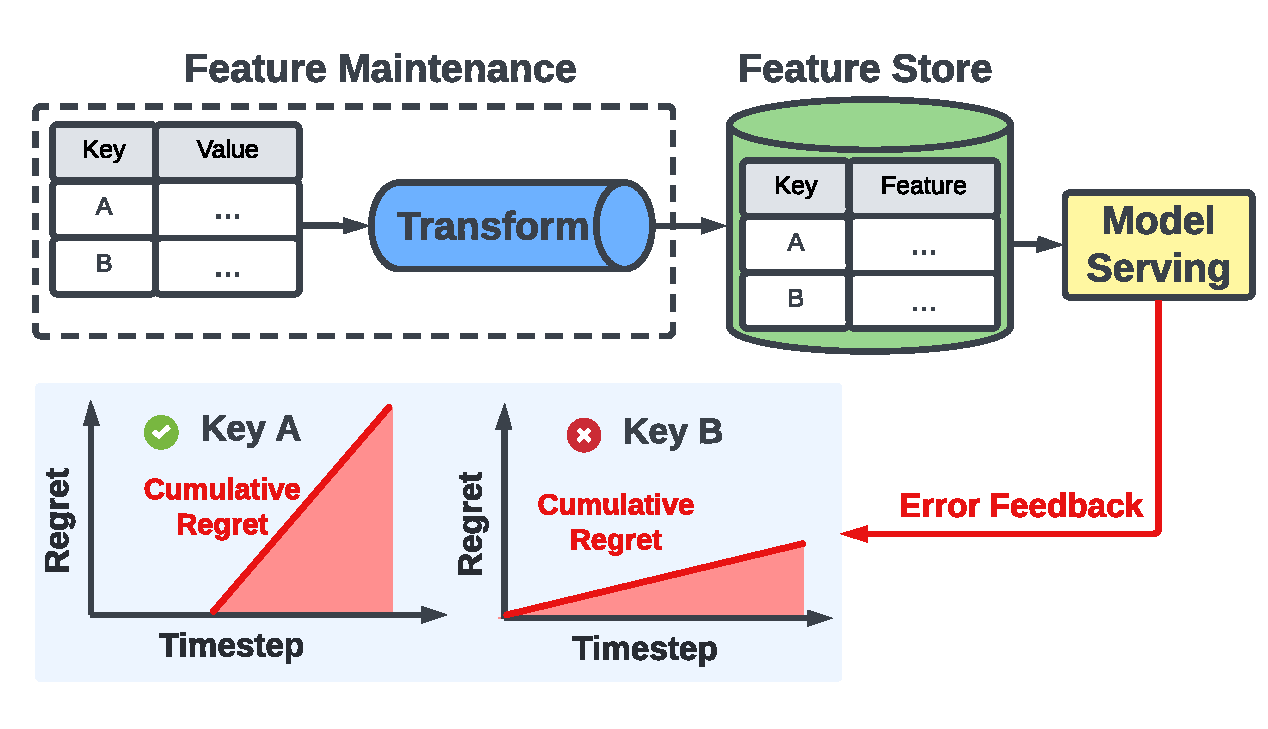
\includegraphics[width=8.5cm]{ralf/figures/overview.pdf}
%\setlength{\abovecaptionskip}{-0pt}
%\setlength{\belowcaptionskip}{-20pt}
\caption{Feature stores serve materialized feature values to downstream models. 
%Computationally expensive feature maintenance pipelines are used to update feature values when the underlying data changes in a best effort fashion.
%However, stale feature values can significantly degrade prediction quality in a manner that depends on the model and feature access pattern. 
\system{} leverage downstream model feedback to prioritize expensive feature updates (\cref{ss:scheduling-policy}).}


\label{f:overview}
\end{figure}

\label{s:introduction}
%This paper describes Ralf, a feature store that explicitly leverages downstream feedback to intelligently schedule feature recomputation.

% \natacha{I find a first sentence that describes the paper, before going into the real intro, to be useful.
% This paper describes Ralf, a feature store that explicitly leverages downstream feedback to intelligently
% schedule feature recomputation}
Most real-world applications of machine learning rely heavily on pre-computed \emph{features} to improve model accuracy and reduce prediction latency.
Features are raw and derived data that are passed as input to machine learning models to capture the context around a prediction.
For example, fraud detection and content recommendation models rely on features describing merchants, users, and content to make accurate predictions. More recently, large language models increasingly depend on features of relevant context (eg. embeddings of past conversational history) to provide more grounded and personalized responses \cite{lee2019latent, guu2020retrieval, packer2023memgpt, lewis2020retrieval}.

%Features include both raw data (e.g., the price of a product) as well as derived data (e.g., a embedding representation of a product) that may require significant computation. 


% \joey{adding a running example really early.}
Consider for example an online news recommendation service that predicts the probability that a specific user will click on specific article.
Standard models for this task \cite{koren2009matrix,DLRM19}
% \joey{cite DLRM and matrix factorization work.}
rely on sophisticated features (such as model based embedding) that summarize the 
user's click history, the text in the article, and the click histories of other users that have clicked on that article.
These features are critical to making good predictions, but are expensive to compute and sensitive to the continuously changing news cycle. 
% \natacha{Not for MLSys, but if we submit elsewhere, it's a little confusing to think of features as part
% of something that is outside of the model, when it feels like it should already been captured in the mode (like the click history, isn't that what you're training on already?) Not for MLSys, but for a less ML heavy conference, might be useful to clarify }
% \joey{In a future cut of this paper we might pull more from section 2 into the introduction to address Natacha's concern}





% In these settings, predictions must be made in 10s of milliseconds but often depend on complex analysis of historical data (e.g., user purchase or click history).
% % in real time. Real-time serving systems are often subjected to tight latency constraints (<100ms), limiting the amount of data retrieval and computation that can be done when a prediction is requested \cite{crankshaw2020inferline}.  
% As a result, prediction serving system often rely on pre-computed \emph{features} (e.g., user purchasing patterns) in addition to query specific inputs (e.g., items in the cart) to provide low-latency, accurate predictions. 

%\joey{This paragraph is good but maybe redundant with the first?  There might be enough example in the above paragraph to drop this one. Actually, the one thing that maybe isn't clear at this point is that features are keyed by the query.}
% Features are derived from computations such as embeddings or large aggregations and often specific to a model query.
% For example, news recommendation models 
% % may use both the current shopping cart items (provided by the prediction request) and a 
% rely on features vectors representing both the historical preferences of each user as well as properties of each article. 
% These feature vectors are typically computed by running historical data through featurization transformations 
% ranging from simple aggregates to complex embedding models.
% When ranking articles for a given user, the features associated with that user and any candidate articles, along with session information are then passed to the news recommendation model.


% However, as users interact with the system the features of both the users and the articles change and those changes often reflect important s


%As users view content their feature

% to encode the historical interests of users and the characteristics of users that click on each article.


% as well as key properties of the hosted content.

% behavior and product ratings into a representative vector. 

Real-time model serving applications, such as online news recommendation services, require low latency predictions, and therefore rely heavily on pre-materialized \emph{feature tables} stored and maintained by a \emph{feature store} to hide the latency associated with deriving features. 
In order to provide low-latency access to important contexual information, \emph{feature tables}
At prediction time, the model serving system 
queries the pre-computed features from the
feature store by specifying a \textit{feature key} (e.g. a user ID), as shown in \cref{f:overview}. 
However, because the features are often derived from data that is constantly changing (e.g., click streams and purchase history), the pre-materialized features also need to be continuously updated with the arrival of new data.
% This process of updating features in response to changing data is the responsibility of the feature store system.
Unfortunately, updating features with every data change can be wasteful and  expensive for high-velocity data streams if the features are not read between updates or cannot be updated incrementally. Beyond computation cost, featurization via third party services also may impost hard rate limits on model-based embedding computations \cite{openai, cohere}. 

\kevin{Discuss potential issues with rate limits also here.
 
 "Beyond computational cost, featurization often uses third party services that impose hard rate limits that constrain the number of featurization updates over a time period. <Add some numbers from common embedding APIs eg. openai, cohere>:"


 https://cohere.com/pricing
 https://platform.openai.com/docs/guides/rate-limits/usage-tiers?context=tier-free

 
 }




% Unfortunately, many of the expensive featurization operations don't have incremental update strategies and so maintaining up-to-date features can be prohibitively expensive.  
% \natacha{You could be more direct here: Existing model
% prediction pipelines are faced with a binary choice
% 1) greedily recomputing features on every input 2) allowing features to become arbitrarily stale. The former is often prohibitive performance-wise while the latter significantly degrades downstream model performance, as shown in Figure 3. 
% This trade-off is not unusual in this space: weakly consistent datastores are faced with similar issues. Relaxing consistency and allowing for stale data can break correctness in ways that are difficult to quantity (cite).  In the specific context of feature stores, however, a third alternative is possible. There exists a clean, measurable metric that one can use as a guide for when and how to compute features:downstream model accuracy. Downstream model accuracy is DEFINE. Using this observation, we can reframe the problem of building a resource-efficient feature store: rather than treating featurisation as ... we can view it as an optimisation problem that seaks to maximise downstream model accuracy. }
%As a consequence, a common solution to feature maintenance is to apply a best effort approach to updating features as new data arrives, which often results in stale or approximated features. 
%While models have some degree of tolerance for stale features, we find that features which are stale or inaccurate often significantly degrade downstream model performance, as show in Figure \cref{fig:staleness}. 

As a consequence, existing feature stores are faced with a choice between (1) greedily processing new updates as they arrive, and (2) allowing features to become arbitrarily stale. 
The former is often prohibitively resource intensive while the latter significantly degrades downstream model accuracy, as shown in \cref{f:staleness}. 
This trade-off is not unusual in this space: weakly consistent data stores are faced with similar issues. In general, relaxing consistency and allowing for stale data can break correctness in ways that are difficult to quantify \cite{sivasubramanian2012amazon,cooper2008pnuts}. 
% \sarah{cite} \jmh{in general}. \natacha{PNUTS, dynamo, cops, tardis, bayou, and a gazillion more}

In the specific context of feature stores, however, ``breaking correctness'' has a measurable metric: \emph{downstream model accuracy}. This is a clean %, measurable 
metric that quantifies the prediction accuracy of a deployed model serving predictions. We can use downstream model accuracy as a guide for when and how to compute features and reframe the problem of building a resource-efficient feature store; rather than treating featurization as a task-agnostic data processing problem, we focus on maximizing downstream model accuracy.

% To address this generality, ``staleness'' in storage systems is often measured in terms of the \emph{number of updates} to a data item, rather than the application-relevant \emph{content} of the updated item.\natacha{See slack for suggested rephrasing}
% In the specific context of feature stores, however, a third alternative is possible. There exists a clean, measurable metric that one can use as a guide for when and how to compute features: downstream model accuracy. Downstream model accuracy measures the prediction accuracy of a deployed model serving predictions.  Using this observation, we can reframe the problem of building a resource-efficient feature store; rather than treating featurization as a task-agnostic data processing problem, we focus on maximizing downstream model accuracy.

We find that the appropriate feature maintenance 
policy for optimizing downstream accuracy can be key-dependent (within a single feature table) and vary across time.
%\natacha{varies across time feels a little strange; it sounds like you're changing the policy itself, rather than when you recompute. We find that deciding when to recompute a feature for optimizing downstream accuracy is both key and time dependent}
Keys that are rarely queried are unlikely to have significant impacts on overall downstream accuracy. 
%Hotspot keys are also frequent in real workloads, as we show in \cref{f:updates_vs_queries}, and do not necessarily correspond to the keys with the most new incoming data. 
Furthermore, even if keys are queried and updated at similar rates, the impact of staleness on accuracy varies dramatically by key. For example, some keys can be updated much less frequently than others without significantly impacting downstream accuracy, as show in \cref{f:update_variance}.
 Prioritizing updates across keys can enable better resource efficiency in optimizing for downstream model accuracy. 


%A stale feature that changes very little with new data or that is rarely queried by downstream tasks is less likely to affect accuracy, offering opportunities for saving on resource cost. 

%, suggesting that the scheduling feature updates should be fine-grained and adaptable. The effect of feature staleness on downstream accuracy can vary between different types of features, or even features within the same feature table.

%A fundamental trade-off with maintaining features is between feature pipeline cost and inference accuracy. Roughly speaking, updating features more frequently reduces the probability of downstream accuracy degradation, but also incurs higher compute resource costs. 



%\sarah{The VLDB paper referred to this as model staleness rather than feature staleness - maybe we can do that do and refer to prior work on data drift?}
%The degree to which feature staleness degrades downstream accuracy can vary between different types of features, or even features within the same feature table. A stale feature that changes very little with new data or that is rarely queried by downstream tasks is less likely to affect accuracy, offering opportunities for saving on resource cost. Existing featurization pipelines use task-unaware, non-adaptable methods for reducing pipeline cost, despite the significant costs incurred by featurization pipelines \cite{lee2018pretzel} \cite{kraft2019willump} and risks of affecting model performance. Resource constrained featurization pipelines use scheduling policies built into streaming systems, and may additionally batch or sub-sample updates to re-compute features less frequently.  We find that the appropriate policy for optimizing downstream accuracy can vary across time and keys (within a single feature table), such as show in Figure \cref{f:key-variance}, suggesting that the scheduling feature updates should be fine-grained and adaptable. 


In this paper, we introduce \system{} (\textbf{r}eal-time, \textbf{a}ccuracy and \textbf{l}ineage-aware \textbf{f}eaturization)
a feature store for real-time, high-density feature updates 
that explicitly leverages downstream feedback to reduce costs with minimal downstream accuracy degradation. We define a metric, \textit{feature store regret}, to estimate accuracy degradation caused by featurization, and present feature update scheduling policies to minimize feature store regret. 

\noindent \textbf{Metrics.} We argue the metric for evaluating a featurization pipeline should be based on downstream task performance. The ability to capture correctness numerically is a unique opportunity in striking  the optimal balance between staleness, computation cost, and accuracy. Specifically, we define \textit{feature store regret}, to measure the drift between the predictions
made with optimal, high-cost features and predictions made with
existing values in the feature store.

\noindent \textbf{Propagating \& Adapting to Feedback.} \system{} leverages knowledge of error feedback from downstream applications to estimate and minimize feature store regret in real-time. \system{} achieves this by tracking the lineage between feature values and downstream predictions, and allowing downstream models to provide error feedback to \system{}. This feedback allows \system{} to prioritise recomputing the features that have the greatest impact on downstream accuracy.


% \noindent \textbf{Propagating \& Adapting to Feedback.}  \system{} leverages knowledge feature query patterns and error feedback from downstream applications to make scheduling decisions. \system{} achieves this by tracking the lineage between feature values and downstream predictions, and allowing downstream models to provide error feedback to \system{}. This feedback allows \system{} to prioritize updates that optimize cost/accuracy tradeoffs in real-time.  
% \natacha{What's the relationship between feature store regret and error feedback? I had assumed that thepe policies would use feature store regret estimation as priority}

% \noindent \textbf{Metrics.} 
% We argue the metric for evaluating a featurization pipeline should be based on downstream task performance. The ability to capture correctness numerically is a unique opportunity in striking  the optimal balance between staleness, computation cost, and accuracy. Specifically, we define a metric, \textit{feature store regret}, to measure the drift between the predictions
% made with optimal, high-cost features and predictions made with
% existing values in the feature store. We use feature store regret to
% evaluate featurization performance offline. \sarah{tie back to "offline evaluation" in later section} \system{} leverages downstream feedback to estimate and minimize feature store regret in real time. %FLAR to prioritise recomputing the features that have the greatest impact on downstream acuracy.

To summarize, we make the following contributions:
\begin{enumerate}
    \item We formalize the feature maintenance problem and define a \textit{feature store regret} metric to evaluate feature store state in terms of downstream accuracy. 
    \item We introduce accuracy-aware feature maintenance policies to reduce the cost of maintaining features while also minimizing the feature store regret. We evaluate these policies with common feature store workloads, anomaly detection and recommendation. 
    \item We implement a system, \system{}, as real-time featurization pipeline that instantiates these policies. We evaluate \system{} at scale with 257,077 keys for the anomaly detection workload to show up to 32.7\% reduction in loss or $1.6\times$ (i.e. 61\%) compute reduction.

\end{enumerate}


\begin{figure}[t]
\begin{center}
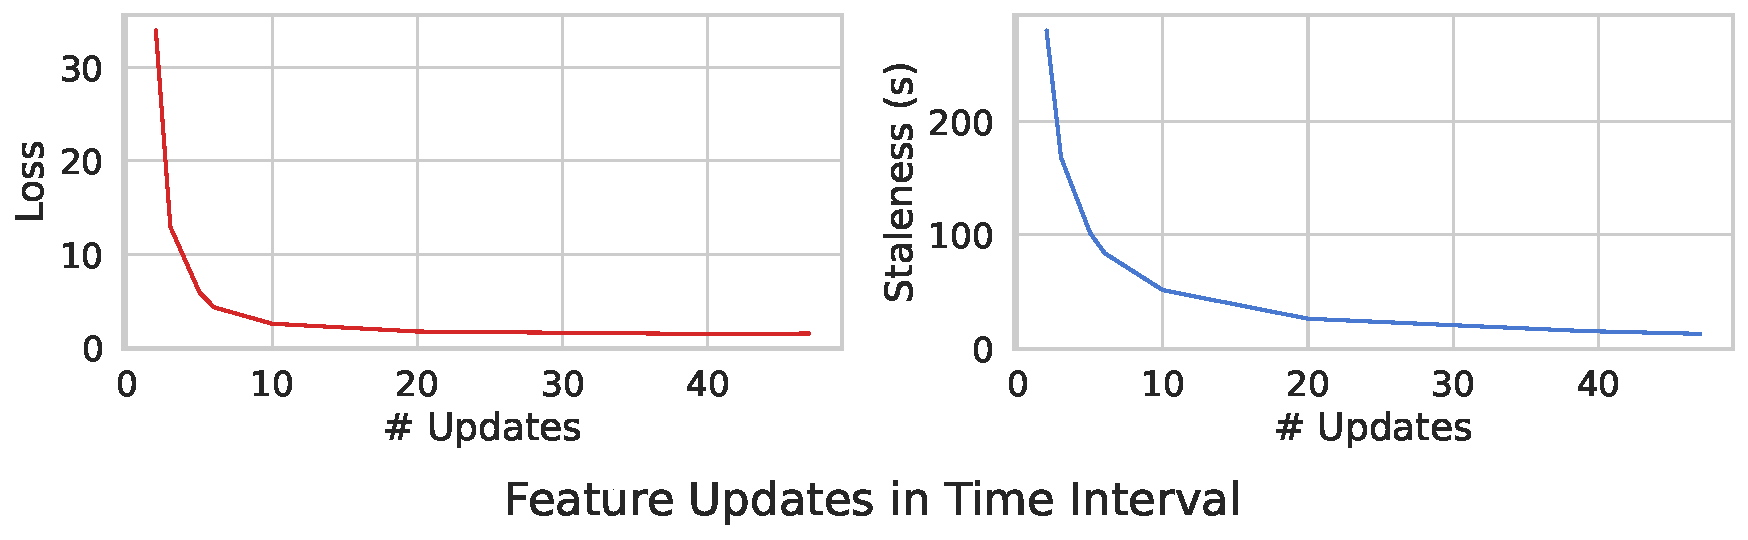
\includegraphics[width=\linewidth]{ralf/figures/loss_staleness_2.pdf}
\centering
\end{center}
 %\setlength{\belowcaptionskip}{-5pt}
 %\setlength{\abovecaptionskip}{-1pt}
\caption{The prediction loss (measured by MASE) on the left is correlated with the feature staleness (time since last update), show on the right. }
\label{f:staleness}
\end{figure}

% \begin{figure}[t]
% \begin{center}
% 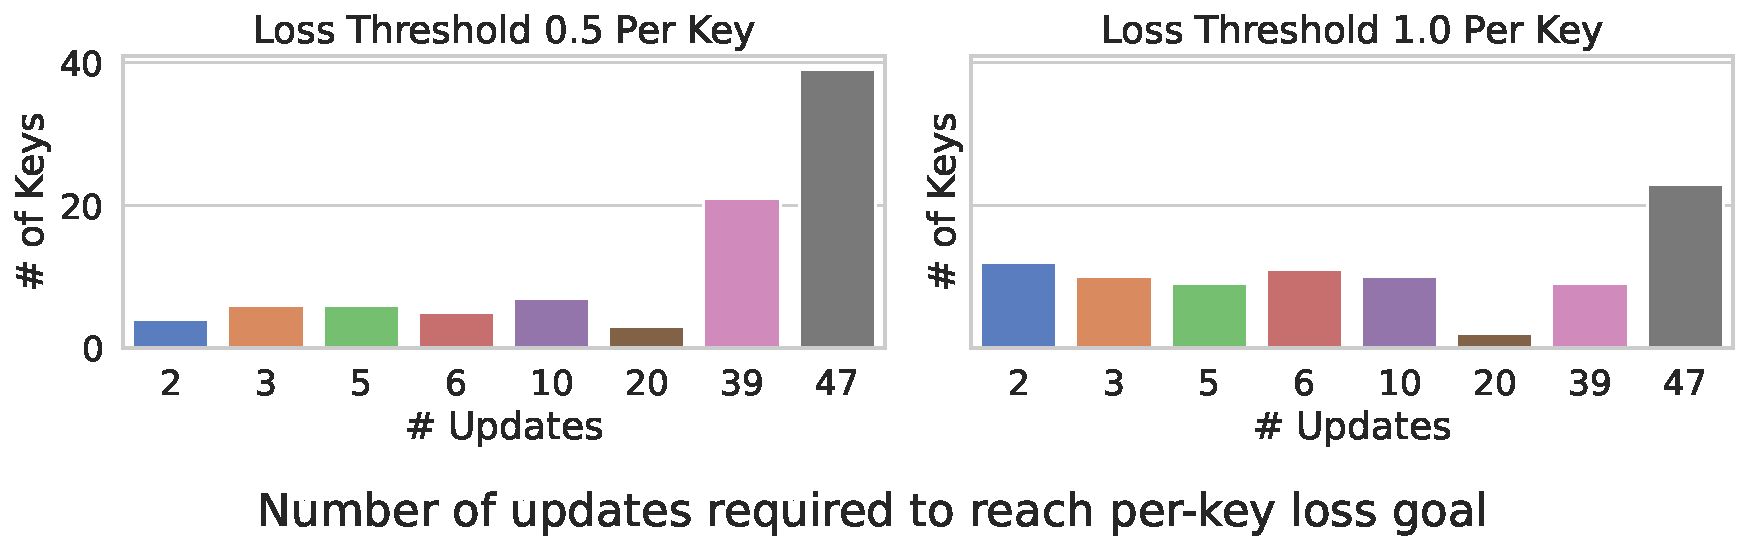
\includegraphics[width=6cm]{ralf/figures/feature_updates.pdf}
% \centering
% \end{center}
%  \setlength{\belowcaptionskip}{-5pt}
% \caption{Distribution of the numbers of feature re-computations required in a time-interval until the accuracy-threshold (0.5 or 1.0) or best accuracy is reached.}
% \label{f:update_variance}
% \end{figure}

% \begin{figure}[t]
% \begin{center}
% 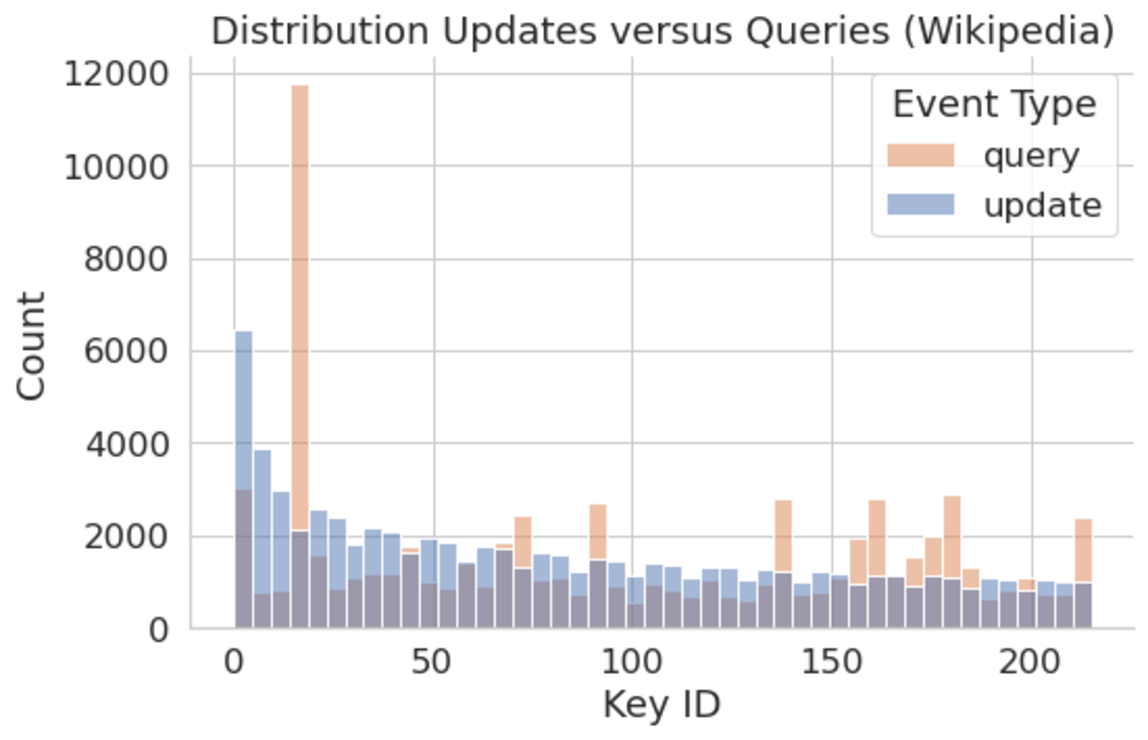
\includegraphics[width=8cm]{ralf/figures/updates_vs_queries.pdf}
% \centering
% \end{center}
%  \setlength{\belowcaptionskip}{-5pt}
%  \setlength{\abovecaptionskip}{-1pt}
% \caption{Distribution of queried keys versus update events to keys for the information retrieval workload (based on Wikipedia document edits and queries collected over a month).}
% \label{f:updates_vs_queries}
% \end{figure}
% \sarah{make figure smaller}
% % %% %---------------------------
% % %---------------------------


% \begin{figure}[t]
% \begin{center}
% 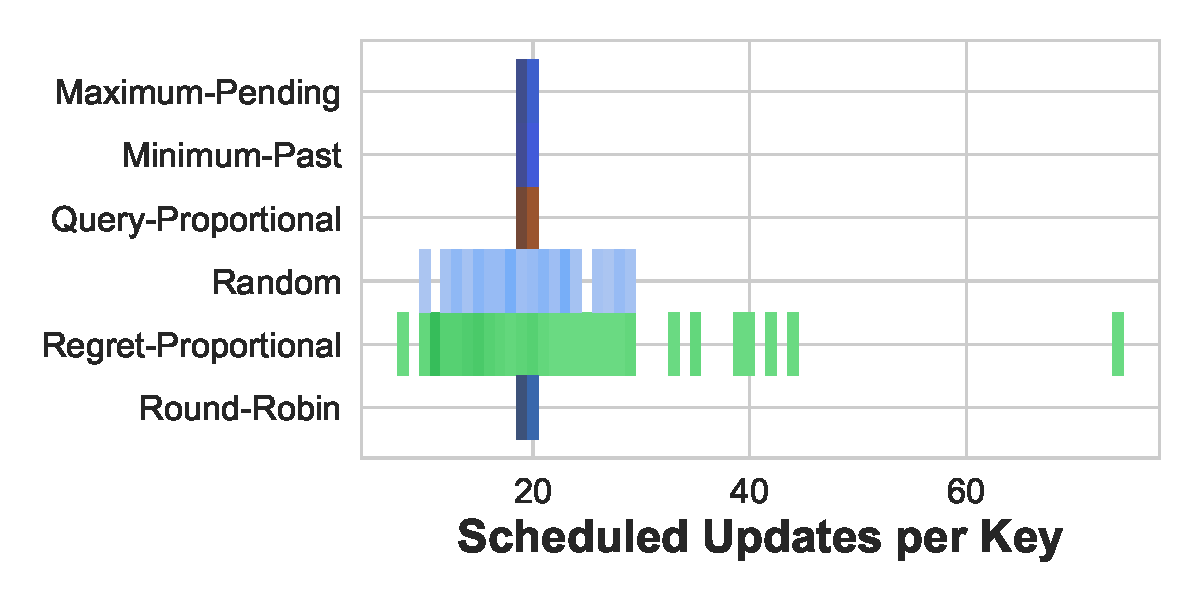
\includegraphics[width=8cm]{ralf/figures/azure_updates_hist_tmp.pdf}
% \centering
% \end{center}
% \setlength{\belowcaptionskip}{-5pt}
% \setlength{\abovecaptionskip}{-1pt}
% \caption{Distribution of featurization updates over keys for baseline (round-robin) versus regret-optimized update scheduling in the anomaly detection workload. Because the rate of raw data updates is uniform across keys, round-robin allocates updates uniformly across keys. The regret-optimize policy is able to non-uniformly distribute updates to reduce downstream error.}
% \label{f:update_variance}
% \end{figure}


% \sarah{recomputations figure: TODO: redo simulation for numbers in this graph bc it looks sus}









%Consider a recommendation model which recommends complimentary products given what a user has already added to their cart. Prior work in prediction serving systems (CITE) would assume that the request-time input is only provided by the query: the products in the cart. However, a real-world model will likely use additional features, such as the user's historical preferences,

%Unlike model training, which is performed relatively infrequently, model inference and pre-processing required features continues to require compute cost for as long as the model is deployed.

% explain more about features!! feature stores. Model serving systems rely on feature stores, contraining features which are expensive to compute. auxilary data. 
% two line starter - get to point. Then go to deeper explanation (look at obladi paper) 

% why is the prioritization unique, or important? we have a clear metric - downstream loss metric that we can compute. in some cases staleness is ok. streaming systems already have a decent amount of studies on deadline. We have a clean way of quantifying how bad the eventual consistency is. 

% Model inference relies on not only prediction input and model weights, but also pre-computed, cached features. Cached features are pre-computed by a separate feauturization pipeline which updates features as new data arrives. Updating features with every data change can be prohibitively expensive when new data is rapidly arriving, and feature operations are compute-intensive. Featurization costs are often controlled by reducing the frequency of re-computing features, resulting in staleness which can impact downstream accuracy. In this paper, we formally define metrics for feature quality in terms of downstream model performance, and introduce policies for optimizing the cost-accuracy tradeoff for maintaining features. 

% In this paper, we study the tradeoff between the compute costs of pre-computing features and the accuracy of the dependent model inference tasks. 


%Machine learning models are increasingly deployed in production to provide personalized and high-quality responses in real-time. 

%Model inference is a core component of many applications, such as e-commerce recommendation and system metric monitoring. Prior work in prediction serving systems (CITE) treats the prediction query as the only input to the model at request time, and the trained model weights as the only parameter impacting prediction accuracy. In reality, model inference relies on additional features generated by a separate featurization pipeline, which typically pre-computes and caches features in a feature store that is queried by the model. The latency of the featurization pipeline can have significant impacts on inference performance, as stale features can degrade prediction accuracy, presenting a tradeoff between featurization costs and downstream model accuracy. In this paper, we explore the cost-accuracy tradeoff of featurization, and develop scheduling policies for streaming featurization using downstream model performance as a metric.  



%
%For example, a model predicting if a user will purchase an item may use an embedding generated from the user's entire history of interactions as additional contextual information. 
%
%


% \textit{Feature Stores} are increasingly becoming a popular design pattern to cache and serve features to models, signifying the need to store pre-computed features. 

%Maintaining features with every new data change is prohibitively expensive, but stale or approximated features can degrade downstream performance. In this paper, we explore the cost-accuracy tradeoff of featurization, and use model inference performance as a metric for evaluating scheduling policies for feature updates. 

%Featurization pipelines are typically separated from inference pipelines, as they are often too expensive to be computed at inference time and must be pre-computed and cached (and models typically have some tolerance for stale features). The latency of the featurization pipeline can have significant impacts inference performance for features which are rapidly changing. 

%Model inference often relies on many different input features, derived with some featurization pipeline. Featurization differs from typical workloads, as features are often pre-computed and cached, and models often have some tolerance for stale features. 



% \textbf{Feature stores signify the need to pre-compute features for low-latency prediction serving systems.}
% Application requirements for real-time predictions constrain the amount of computation that can be done on-request, as inference-time computations must meet tight latency SLOs (CITATION). Real-time prediction serving systems often query an \textit{online feature store} for additional features at inference time. Feature stores are becoming a popular design pattern in industry to enable models to incorporate a features that would be otherwise to expensive to compute. 

% % Models can take advantage of many different features to improve prediction accuracy, such as low-dimentional representations (e.g. embeddings) of additional data. 
% %The need for feature stores come from real-time model serving applications, which must meet tight latency SLOs (CITATION) (<100ms) that constrain the amount of computation which can be performed on-request.
% % Prediction performance depends BOTH the quality of the trained model AND the quality of the pre-computed features. Featurization pipelines should be optimized for downstream model performance.  




% \textbf{Featurization is very expensive - need to determine when to update what }
% \begin{itemize}
%     \item Data updates can be a rapid stream - e.g. user clickstream 
%     \item Updating with every new event is prohibitively expensive - while materializing on-the-fly is too high latency 
%     \item Featurization operators are often not incremental - e.g. computing an language embedding from text that is edited multiple times 
% \end{itemize}

% \textbf{Reducing featurization costs involves accuracy degregation}
% Meeting cost constraints for featurization pipelines often results in performance degredation of the downstream model. A standard protocol to reducing featurization cost is \textit{feature approximation}, where features are approximated by reducing the frequency of re-computation or sub-sampling updates. While models have some degree of tolerance for feature approximation, we find that features which are stale or inaccurate often significantly degrades downstream model performance. As a result, feature maintenance introduces a trade-off between
% \one{} the \textit{cost} of the featurization pipeline, and
% \two{} the \textit{accuracy} of the downstream application performance. 

% \begin{itemize}
%     \item Statistical - not all or nothing 
%     \item Featurization costs are usually reduced by decreasing the frequency of processing feature updates - e.g. dropping updated or increasing window size 
%     \item Models have some degree of tolerance for feature approximation - but eventually performance will degrade  
%     \item As a result, feature maintenance introduces a trade-off between
% \one{} the \textit{cost} of the featurization pipeline, and
% \two{} the \textit{accuracy} of the downstream application performance. 
% %
% \end{itemize}

% Scheduling and load shedding policies for data processing systems used for streaming featurization (e.g. Flink, SparkStreaming) are oblivious to their impact on downsteam model performance. Streaming systems don't natively include mechanisms for adapting to feedback from downstream quality metrics. Scheduling and load shedding policies don't consider the statistical nature of models serving. Defining dependencies between features, as well as between queried features and downstream model performance, is also challenging with existing stream system APIs, making it difficult to propagate feedback on downstream model performance to the correct subset of upstream features. 

% \\
% \\

% % Setup:
% % ML models in complex pipelines that respond to requests in real-time.
% Machine learning models are increasingly deployed in production to provide
% personalized and high-quality responses in real-time.
% %
% The deployment of such models at scale requires the creation of complex pipelines
% which preprocess raw data into \textit{features}, which are fed to a model to generate
% predictions.
% % 
% To meet real-time latency constraints (often <100ms),
% \peter{need citation}
% an emerging pattern in industry combines both streaming and storage systems into a
% \textit{feature store}, which is responsible for serving pre-computed features to models.
% %

% %
% By querying the feature store, models can quickly retrieve features that may be too expensive
% to compute upon request.
% %
% For example, recommendation models may use expensive embeddings that are generated
% from a user's browsing history.
% %
% Querying the browsing history and computing the embeddding at inference time may
% violate tight latency SLOs.
% %
% Instead, the embedding can be pre-computed and cached in a feature store,
% which enables fast responses from the recommendation model.
% %

% %
% Caching introduces the new problem of how features should be \textit{maintained} over time.
% %
% While feature stores may provide fast responses, the returned features may grow
% \textit{stale}, or inconsistent with the latest data.
% %
% Stale features can hurt model performance as they become too out-of-date or miss
% important updates.
% %
% These inconsistencies are especially problematic in the presence of
% \textit{downstream features}, which are features derived from other features,
% because the feature store may serve sets of features which are inconsistent with one another.
% %
% While recomputing features whenever data arrives reduces staleness, these recomputations
% become prohibitively expensive when processing high volume streams or running
% expensive featurization transformations.
% %

% %
% As a result, feature maintenance introduces a trade-off between
% \one{} the \textit{cost} of the featurization pipeline, and
% \two{} the \textit{accuracy} of the downstream application performance. 
% %
% Existing techniques use approximation to reduce cost, but significantly impact accuracy.
% %
% Batching updates (e.g. by assigning updates to a sliding window)
% reduces the frequency of recomputation, but results in stale features.
% \peter{Should mention efficiency, e.g. feeding a batch into a model is cheaper than
% computing one at a time.}
% %
% Sub-sampling updates reduces the number of updates to process, but results in data loss.
% %
% Thus, approximation may reduce the quality of features which may affect the performance
% of the overall pipeline.
% \peter{need citations}
% %

% %
% In contrast, a system can leverage application-level performance metrics to navigate
% the tradeoff between accuracy and cost.
% %
% In this paper, we formalize the problem of feature maintanence as a scheduling problem
% in which updates are scheduled to maximize application performance under cost constraints.
% %
% We evaluate existing scheduling policies for streaming systems in the context of
% feature maintenance.
% %
% We design an adaptive scheduling policy which uses query patterns and information about
% feature dependencies to prioritize updates.
% %
% We evaluate our contributions in
% \textit{Ralf} (\textbf{r}eal-time, \textbf{a}ccuracy, and \textbf{l}atency-aware \textbf{f}eaturization), our prototype featurization pipeline which maintains multiple
% interdependent \textit{feature tables} over streaming updates.

% The rest of the paper is organized as follows:
% \peter{TODO: fill this in with summaries of each section}


% Machine learning models are increasingly being deployed the serve predictions in real-time. Real-time serving systems are often subjected to tight latency constraints (<100ms), limiting the amount of data retrieval or computation that can be done when a prediction is requested. A common design pattern in industry machine learning pipelines is to deploy a \textit{feature store}, responsible for storing and serving pre-computed features to models. 

% fundamental question - how should data changes to propagated? or given that some parts of a computation can be cached, have varying latency, etc. how can we schedule maintenance? 

% Data processing steps in ML pipelines are also typically expensive (such as aggregations over large amounts of data, or model predictions) 
% two questions: what should be materialized, and what should be cached - OR just the question - what upstream updates should be materialied when 
% Updates to raw, upstream data sources must propagate to downstream, derived data, known as "features". 

% How are features computed? Why are we compute-bound? Introduce notion of accuracy to
% optimize compute.
% Features are typically computed either
% \one{} \textit{eagerly} where raw data is immediately processed into features, or
% \two{} \textit{lazily} where features are generated in response to a query.
% %
% Eager computation ensures low-latency responses at the cost of more resources,
% whereas lazy computation uses just enough resources to respond to queries but may
% result in higher response times.
% %
% While eager computation may meet the latency constraints of real-time machine learning
% pipelines, the resource intensive nature of machine learning workloads may be
% prohibitely expensive.
% %
% Thus, feature stores need to pursue a best-of-both-worlds approach and identify
% high-priority features to compute eagerly to ensure low response times,
% and lazily processing low-priority features to reduce costs.
% %
% 
% %
% Choosing which features to compute eagerly introduces new challenges related to
% feature \textit{maintenance}.
% %
% Features derived from high volume data streams, such as e-commerce clickstreams
% or system logs, constantly receive new data.
% %
% \textit{Downstream features}, which are derived from previously-computed upstream features,
% grow stale and may affect overall pipeline performance if features become too out-of-date
% or miss important updates.
% %


%
% Pre-computed, cached features allow real-time models to query for contextual features at inference time which would otherwise be too expensive to compute on-request. For example, a model predicting if a user will purchase an item may use an embedding generated from the user's history of interactions as an additional feature. Querying the user's historical data and calculating the embedding at inference time could violate tight latency SLOs. Instead, the embedding can be pre-computed and cached in a feature store, so the model can query the user's embedding when making a prediction. 

%The feature store is responsible for versioning features to ensure feature transformations are used across training and inference time, and responding to feature query requests with sufficiently low latency (usually through storing features in an in-memory database). 

% Caching features introduces new challenges. Slight changes to the featurization transformations can cause dramatic performance degregations for downstream model predictions due to data drift, unless the model is re-trained with the new version of the features. Features are often generated from upstream data sources, which may be rapidly changing (such as with streaming data sources). Features need to be maintained by processing upstream updates. However, re-computing features for every new update can be prohibitively expensive for high-density streams of updates running through expensive featurization transformations. 

% Caching features introduces the problem of how cached features should be \textit{maintained} with new data. Features derived from data streams, such an e-commerce clickstream or system logs, are constantly receiving new data. As new data arrives, downstream features grow stale, and can hurt downstream model performance if features grow too out-of-date or miss important new updates. However, re-computing features for every new update can be prohibitively expensive for high-density streams of updates running through expensive featurization transformations. 

% Existing streaming featurization pipelines reduce compute costs with feature "approximation", such as by batching or sub-sampling updates. Batching or windowing updates reduces the frequency of re-computation, but results in staler features depending on the window size or the time between batches. Sub-sampling updates reduces the number of updates that need to be processed, but results in data loss. Approximation can reduce the quality of features and degrade downstream performance, as features will be less fresh or missing data. 

%In addition, processing upstream updates it not always beneficial, such as if the feature being updated is never queried, or if the feature is unlikely to change. 

%Caching features introduces the problem of how cached features should be \textit{maintained} with new data. The raw data sources which features are derived from are often rapidly changes, such as in cases where features are derived from aggregating over data streams. Features are generated from transforming one or more upstream data sources (or even other features). Updates to upstream data should be propagated to be reflected in downstream features by re-computing the features with the new data. However, re-computing features for every new update can be prohibitively expensive for high-density streams of updates running through expensive featurization transformations. 

% \begin{figure}[t]
% \begin{center}
% \includegraphics[width=8cm]{ralf/figures/fake graph.png}
% \centering
% \end{center}
% \caption{\label{fig:vectors} Feature store overview. }
%     \label{f:feature-store-overview}
% \end{figure}



%Despite the importance of features for downstream model performance and the significant cost of feature updates, there are few policies for scheduling feature updates. 



% As a result, feature maintenance introduces a trade-off between (1) the \textit{cost} of the featurization pipeline, and (2) the \textit{accuracy} of the downstream application performance. Managing this tradeoff is an unexplored problem, and current featurization pipelines lack metrics to provide feedback on feature quality. Existing metrics for optimizing schedulers for data streaming or query processing are insufficient for featurization pipelines, which ideally should be optimizing for performance of the downstream task. Associating upstream data updates and downstream queries is difficult without clear dependencies defined between features, which can be defined in terms of multiple other data sources and features.



%Existing metrics for optimizing schedulers for data streaming or query processing are insufficient for featurization pipelines, which ideally should be optimizing for performance of the downstream task. Feature stores may contain multiple interdependent features which all require varying degress of freshness. 

% interdepe


%Most feature stores focus on the data drift challenge through versioning features, managing feature metadata, and synchronizing features used in training and inference pipelines,  


%Features computations are often high latency and compute intensive. For example, a user preference embedding may require querying a user's entire history of interactions and running the history through an expensive embedding model. For such features to be used for online predictions with tight latency constrains, the features must pre-computed and cached. Cached features must still be updated with underlying data changes, such as new user interactions. However, re-computing features for every new event can be prohibitively expensive. Featurization costs are typically reduced by approximating features, such as by reducing the frequency of re-computation, such as with windowing, batching, or sub-sampling updates. Approximation can reduce the quality of features and degrade downstream performance, as features will be less fresh or missing data. 

% Our work introduces a featurization pipeline which is both quality and query aware to maximize downstream inference performance. In this paper, we make the following contributions: 
% \begin{itemize}
%     \item We formalize the problem of feature maintenance in terms of maximizing downstream application performance under cost constraints.
%     \item We evaluate existing load shedding and prioritization policies for streaming systems in the context of feature maintenance. 
%     \item We design an adaptive scheduling policy which uses query pattern and feature dependency information to prioritize updates.
%     \item (Learned scheduler thing?) 
%     \item We build a prototype featurization pipeline, \textit{Ralf} (realtime, accuracy and latency-aware featurization), which maintains multiple interdependent \textit{feature tables} over streaming updates. Ralf tracks update and query patterns over feature keys to propagate to schedulers.  
% \end{itemize}
% 
